\section{Adaptive Offloading Controller Design}
\label{sec:Off_Ctlr}
In this section, we present the computation offloading controller design for automotive control applications that leverages cloud. This approach enables dynamic switching between and on-board and remote resources based on the control application specification and current network conditions.

In the mobile cloud computing area, cloud-based augmentation techniques \cite{ref:MCC_aug, ref:cloudlet} and computation offloading problem \cite{ref:MCC_survey1, ref:MCC_survey2} have been extensively studied. However, major emphasis is placed on saving energy on mobile devices and computation offloading is largely determined by the viability of network conditions at any given point of time. In the automotive domain, however, the most important consideration is satisfying the real-time constraints of the control applications. A typical control loop in an application like adaptive cruise control (ACC) takes 10 ms. This, given the current network communication standards, makes it infeasible to offload core control computation to the cloud. Therefore, we need to identify parts of control computation that are amenable for offloading to the cloud without compromising on the safety and stability of the system. The candidate computational part must have a delay tolerance in the range of 150-200 ms and potentially benefit from additional computation resource and/or data accessed via cloud. 

\begin{figure}
%\hspace{0.2in}
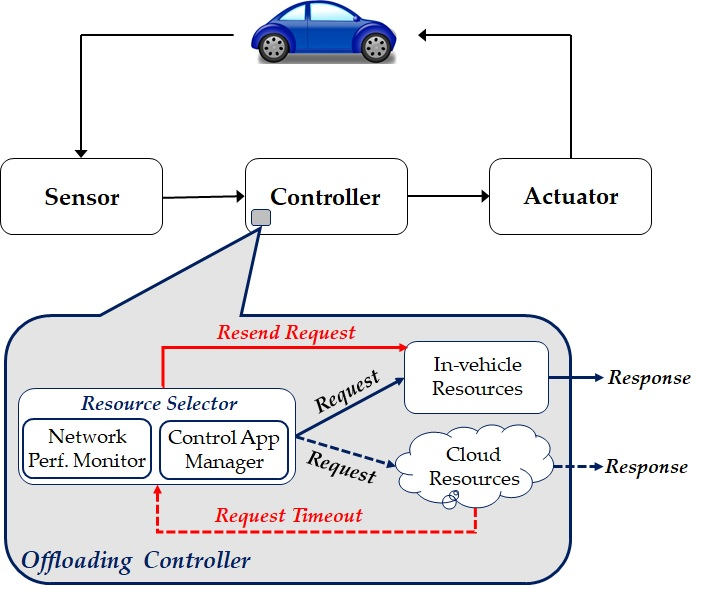
\includegraphics[width=3.25in,height=3in]{off_ctlr.jpg}
 \caption{Computation Offloading Controller Architecture \label{fig:OFF_CTLR}}
\end{figure}

Figure \ref{fig:OFF_CTLR} shows our offloading controller architecture design for control applications. The basic functionality of the offloading controller is to determine whether to execute a given computational task on local or remote resource. The decision-making process relies two components, namely, Network Performance Monitor and Control Application Specification. The network performance monitor component continuously monitors the network characteristics such as available bandwidth and uplink data rate. The control application specification component identifies the self-contained parts of control computation (e.g., pre-processing sensor data, vehicle state estimation) and their computational and latency requirements. These parts are specified as tasks and this task specification along with the current network conditions guide the process of selecting a resource. Once a suitable resource for a given task is identified, the task is executed on the resource and the response is fed to the control loop. 

\begin{algorithm}
\;
\tcc{Computation task ${T_{i}}$ = $(S_{i}, C_{i}, L_{i})$  where,\\
\hspace{0.3in}$S_{i}, S_{i}^{\prime}$: size of the input \& output data \\
\hspace{0.3in}$C_{i}$: \# of CPU cycles required for task  ${T_{i}}$ \\
\hspace{0.3in}$L_{i}$: latency requirement of the task ${T_{i}}$ \\
$C_{cloud}$: \# of CPU cycles available in the cloud \\
$\beta, \beta^{\prime}$: available uplink and downlink data rate \\
$T_{i}^{rsrc}$: resource to which the task {\em i} is assigned 
}
\;
 \SetKwInOut{Input}{Input}
 \SetKwInOut{Output}{Output}
\Input {Set of input tasks $\mathcal{T}=\{T_{i}\}, i=1,2,...,n$}
\Output {Task execution output: {$T_{i}^{out}$}}

\caption{Computation offloading: high-level steps}
\label{alg:off_ctlr}
\;
\begin{algorithmic}
\WHILE{$\mathcal{T} \neq $ NULL}
\STATE {\textbf{\underline{measure}}} available uplink data rate for task $T_{i}$: $\beta$
\STATE {\textbf{\underline{estimate}}} network delay: $\delta_{i}^{net}$ := $\frac{S_{i}}{\beta}$ + $\frac{S_{i}^{\prime}}{\beta^{\prime}}$
\STATE {\textbf{\underline{estimate}}} computation delay: $\delta_{i}^{comp}$  := $\frac{C_{i}}{C_{cloud}}$  \;
\IF {$\delta_{i}^{net}$+$\delta_{i}^{comp}$ $<$ $L_{i}$}
\STATE $T_{i}^{rsrc}$ := {\em cloud} 
\ELSE
\STATE $T_{i}^{rsrc}$ := {\em on-board} 
\ENDIF
\STATE {\textbf{\underline{execute}}} task on $T_{i}^{rsrc}$ and \textbf{return} $T_{i}^{out}$
\IF {$T_{i}^{rsrc}$ == cloud $\land$ timeout}
\STATE {\textbf{\underline{execute}}} task $T_{i}$ on {\em on-board} resource and \textbf{return} $T_{i}^{out}$
\ENDIF 
\ENDWHILE
\end{algorithmic}
\end{algorithm}

Algorithm \ref{alg:off_ctlr} describes the step-by-step process of resource selection and offloading. When the cloud resource is selected for task execution and the input data is offloaded to the cloud, the response might not come back within a desirable timeframe (say, for example, due to temporary resource outage). In such cases, the request timeout will get triggered and the same request will now have to be forwarded to the local resource. As pointed out in Section II, due to limited understanding of the surrounding context in the local-only case, the response generated by the local resource may be less efficient (in terms of time taken for task execution and/or the quality of control output) compared to a cloud-based approach. In the tradeoff analysis, particularly in a feedback control system in the automotive domain, the emphasis is more on the stability of the system than quality of output in one control step as compromising on stability could lead to undesirable consequences.